\documentclass[12pt]{article}

% Packages
\usepackage[utf8]{inputenc}
\usepackage{amsmath}
\usepackage{amssymb}
\usepackage{graphicx}
\usepackage{hyperref}
\usepackage{geometry}
\usepackage{float}

% remove the indent at the beginning of a paragraph:
\setlength{\parindent}{0pt}

% Line spacing
\renewcommand{\baselinestretch}{1}

% distance between new paragraphs:
\setlength{\parskip}{0.5em}

% Title design:
\usepackage{titling}
\pretitle{\begin{center}\LARGE\bfseries}
\posttitle{\par\end{center}\vspace{-0.5em}}
\preauthor{\begin{center}\large}
\postauthor{\par\end{center}\vspace{-2em}}
\predate{\begin{center}\large}
\postdate{\par\end{center}\vspace{-1em}}


% Geometry settings
\geometry{
    a4paper,
    total={170mm,257mm},
    left=20mm,
    right=20mm,
    top=20mm,
    bottom=20mm,
}

% Set the figure counter to reset within subsections
\counterwithin{figure}{subsection}

% Document
\begin{document}

% Title Page
\title{Homework 1: Vector Search}
\author{Naomi Derel 325324994, Gili Cohen 326280815, Renana Shachak 213920010}
\date{02.07.2024}
\maketitle

% % Table of Contents
% \tableofcontents
% \newpage

% Sections
\section{Faiss}

With permission from the course staff, we kept our answers for the original question and not the updated requirements, as we finished it prior to the update.

\subsection{Running Times}

\begin{figure}[H]
    \centering
    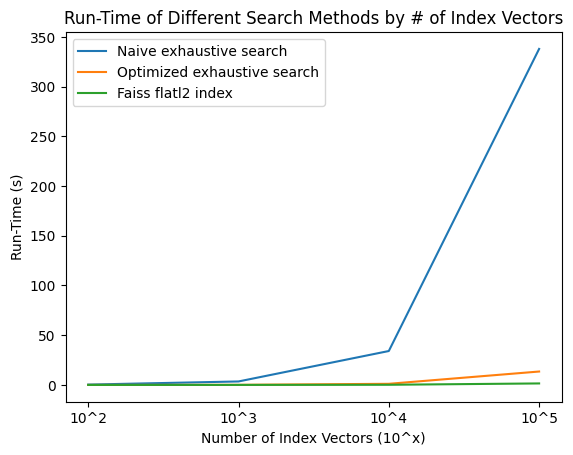
\includegraphics[width=0.8\textwidth]{images/1_1_1.png}
    \caption{Running times by Number of Index Vectors}
\end{figure}

\begin{figure}[H]
    \centering
    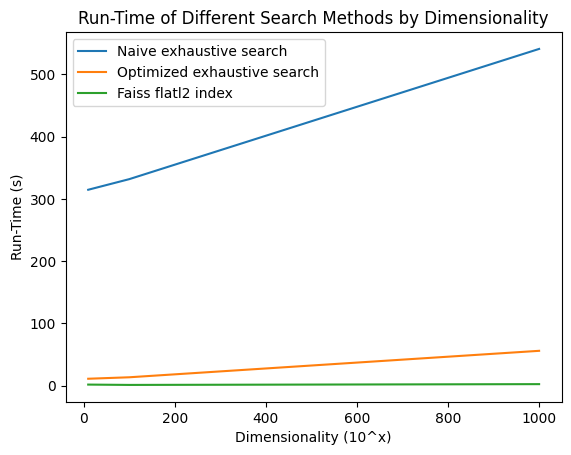
\includegraphics[width=0.8\textwidth]{images/1_1_2.png}
    \caption{Running times by Dimentionality}
\end{figure}

\subsection{Faiss LSH}

\begin{figure}[H]
    \centering
    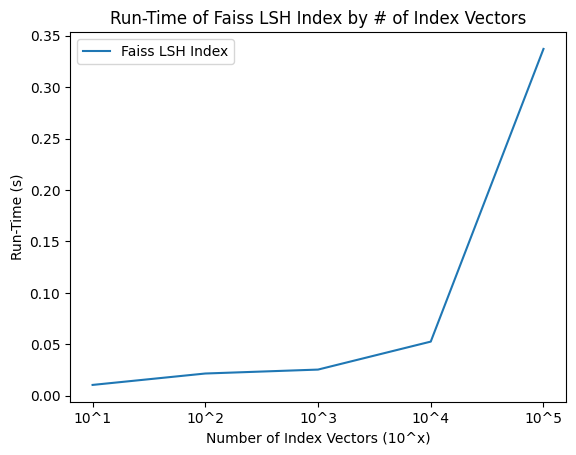
\includegraphics[width=0.8\textwidth]{images/1_2_1.png}
    \caption{Running times by Number of Index Vectors}
\end{figure}

\begin{figure}[H]
    \centering
    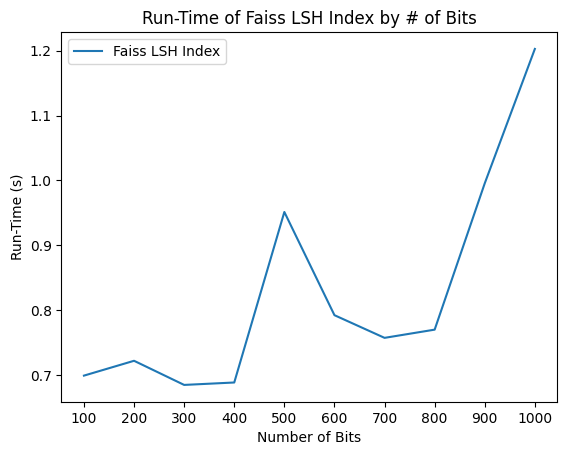
\includegraphics[width=0.8\textwidth]{images/1_2_2.png}
    \caption{Running times by Number of Bits}
\end{figure}

\begin{figure}[H]
    \centering
    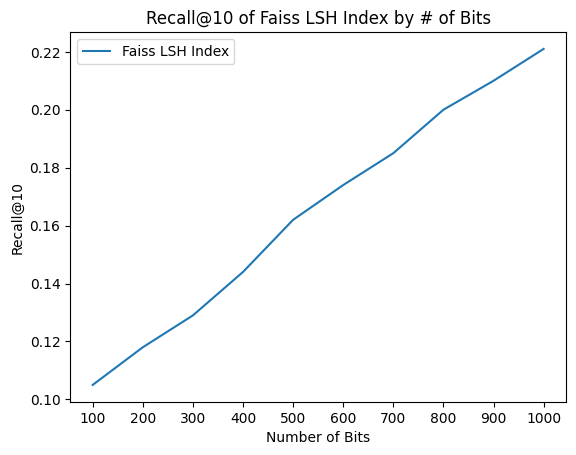
\includegraphics[width=0.8\textwidth]{images/1_2_3.png}
    \caption{$Recall@10$ by Number of Bits}
\end{figure}

\newpage

\section{Implementing an Index}

\subsection{LSH vs. Native Exhaustive Search}

\begin{enumerate}
    \item Running time of the \texttt{semi optimized exhaustive search} function was: \textbf{4.14 seconds}.
    \item Running time of building the LSH index was: \textbf{0.62 seconds}.
    \item Running time of LSH search over query vectors was: \textbf{0.13 seconds}.
    \item $Recall@10$ for the LSH index was: \textbf{0.138}.
\end{enumerate}

\subsection{Custom Indexing Algorithm}

\subsubsection*{Implementation Description}

For our solution, we decided to implement an index based on the HNSW algorithm we saw in the lecture. 
Our intuition for this choice comes from the assumption that the HNSW is a very fast algorithm based on the skip-list data structure, and yet it is more accurate than the LSH algorithm.

We supported this intuition by testing the implementation of the HNSW algorithm in the Faiss library, and found that an ideal implementation can reach the 0.8 recall@10 mark in a very short time.

For our implementation, we...

\subsubsection*{Performance Measures}

\begin{itemize}
    \item \textbf{creating custom indexing algorithm:} x seconds, half the time of section 2.1.2
    \item \textbf{searching with custom indexing algorithm:} x seconds, a third of the time of section 2.1.3
    \item \textbf{recall@10 for custom indexing algorithm:} x, at least 0.8
\end{itemize}



\newpage

\section{Pinecone VectorDB and RAG}

\subsection{Dataset Selection}

We opted to use the Stanford Question Answering Dataset (SQuAD) as the dataset for this task. 
It consists of questions posed by crowdworkers on a set of Wikipedia articles, with corresponding reading passages.
In total, SQuAD 1.1 contains 100,000+ question-answer pairs on 500+ articles.

The segments of contexts are repeated across questions, and after eliminating duplicates, we are left with 20,958 unique contexts.
The segments are relatively short, with most segments containing less than 200 words, and the longest one being 635 words.

The answers for the questions are usually short, precise answers that can be found in the context, which makes them potentially easier to compare with the generated answer. However, there are also some questions that do not have an answer in the context.

The rationale behind choosing SQuAD is that it is a well-known dataset for QA tasks, but as we saw in a preliminary analysis, it contains a variety of "trivia-like" questions of lesser known topics, which we quickly became convinced could mislead a regular QA model.

\subsection{Anecdotal Model Evaluation}

The standard QA model from cohere may fall short in answering factual questions in specific domains it might have not been exposed to enough. We present a few anecdotal examples of such cases:

\begin{enumerate}
    \item \textbf{Question:} The College of Science began to offer civil engineering courses beginning at what time at Notre Dame?
    
    \textbf{Correct Answer:} the 1870s.
    
    \textbf{(Shortened) Response without RAG:} The College of Science at the University of Notre Dame began offering civil engineering courses in the fall of 2019. This expansion of the college's curriculum was part of a broader effort to enhance the university's engineering programs\dots

    \textbf{Response with RAG:} The College of Science at Notre Dame began offering early courses in civil and mechanical engineering in the 1870s.
    
    Clearly the response without RAG is very far off.

    \item \textbf{Question:} How many departments are within the Stinson-Remick Hall of Engineering?
    
    \textbf{Correct Answer:} five.

    \textbf{Response without RAG:} There are six departments within the Stinson-Remick Hall of Engineering: 
    Aerospace and Mechanical Engineering,
    Chemical and Biomolecular Engineering,
    Civil and Environmental Engineering and Earth Sciences,
    Computer Science and Engineering,
    Electrical Engineering,
    Materials Science and Engineering 

    \textbf{Response with RAG:} There are five departments of study within the College of Engineering, which is housed in the Fitzpatrick, Cushing, and Stinson-Remick Halls of Engineering.

    The response without RAG gave detail and seem to have invented a department. The response with RAG is more concise and accurate.

    \item \textbf{Question:} How many student news papers are found at Notre Dame?
    
    \textbf{Correct Answer:} three.
    
    \textbf{(Shortened) Response without RAG:} There are two student newspapers at the University of Notre Dame: 
    1. The Observer: This is the main student newspaper on campus...
    2. Irish Insider: This is a student-run sports newspaper that focuses specifically on Notre Dame athletics...

    \textbf{Response with RAG:} There are three student newspapers at the University of Notre Dame: The Observer, Scholastic, and The Juggler.  

    The response without RAG is missing a newspaper, which might be due to a later addition of the paper or because of lacking information. 
\end{enumerate}

\subsection{RAG Pipeline}

\begin{itemize}
    \item \textbf{Document reading and preprocessing:} We retained all the contexts from the SQuAD dataset, both in training and evaluation, into our corpus. We avoided duplicate snippets (most passages have multiple questions), and were left with 20,958 unique contexts.
    We embedded these documents using the \texttt{all-MiniLM-L6-v2} model, as shown in the tutorial.
    
    \item \textbf{Chunking documents for embedding generation:} As described in "dataset selection", the contexts for the questions are passages from Wikipedia articles, and so they are relatively short (we could think about this as if the passages are already pre-chuncked documents).
    Due to this, we believe further chunking might cause more loss of information than gain in noise reduction.
    
    \item \textbf{Embedding generation and insertion into Pinecone VectorDB:} We created a Pinecone VectorDB index using the API Key, and upserted the embeddings of the pure text of the documents into the index. 
    In our dataset, we chose not to include additional metadata, as it was not informative further than the text itself.
    
    \item \textbf{Retrieval of relevant documents:} Given a specific query, we encode it and use the index to retrieve the top $k$ most similar documents (we used $k=3$). We combined the documents into a single source knowledge string.

    \item \textbf{Generating answers to given questions using the retrieved documents:} we augmented the query with the source knowledge and query strings in the following way:

\begin{verbatim}
Using the contexts below, answer the query.
Contexts: {source_knowledge}. If the answer is not included in the source 
knowledge - say that you don't know.
Query: {query}
\end{verbatim}

    We input the augmented query into the Cohere \texttt{command-r-plus} model to receive a response.

\end{itemize}

\subsection{Insights}


The examples shown present multiple potential types of error: blatantly incorrect information (ex. 1), hallucinated information (ex. 2) or lacking information (ex. 3).
The common theme among these examples are domain specific, factual questions - which is what we aimed to solve with RAG.

We also conducted a small-scale evaluation of the RAG pipeline on a few (50) examples, and found that the RAG model, including the retrieval step, was faster than the standard QA model. 
We explain this by suggesting that the regular model without context might take longer to generate an answer it doesn't necessarily know, while the RAG model can answer very quickly once the context is provided.

Additionally, as supported by the examples we managed to fix, the average cosine similarity between the generated response and the answer was higher using RAG than the QA model.

% insert image:
\begin{figure}[H]
    \centering
    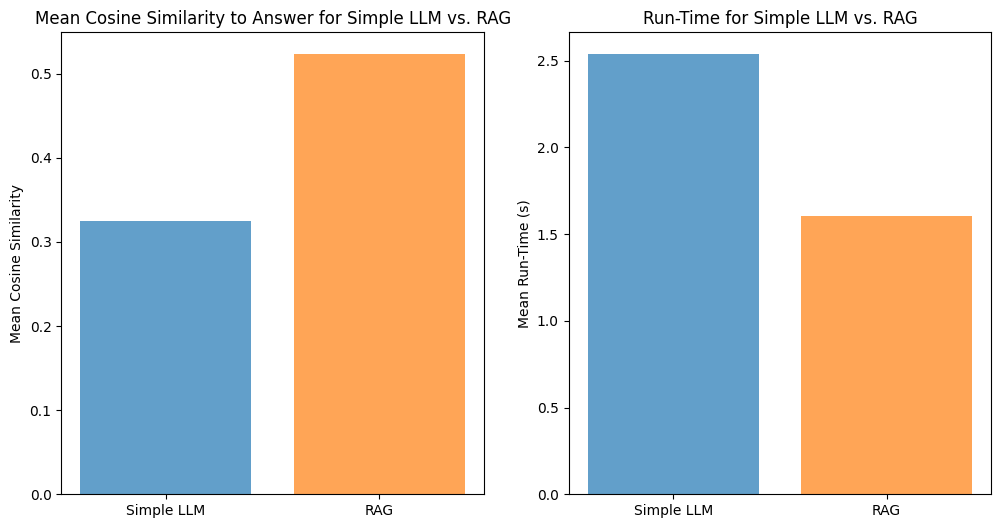
\includegraphics[width=0.8\textwidth]{images/3_1.png}
    \caption{Comparison of RAG and QA model on 50 examples}
\end{figure}

% % Bibliography
% \newpage
% \begin{thebibliography}{99}
%     \bibitem{ref1} Author, \emph{Title}, Publisher, Year.
%     \bibitem{ref2} Author, \emph{Title}, Publisher, Year.
%     % Add more references as needed
% \end{thebibliography}

\end{document}